\chapter{Traiettorie}

L'obiettivo del \textbf{trajectory planning} è quello di creare l'input di riferimento al sistema di controllo del movimento del robot. \\
\begin{figure}[H]
	\centering
	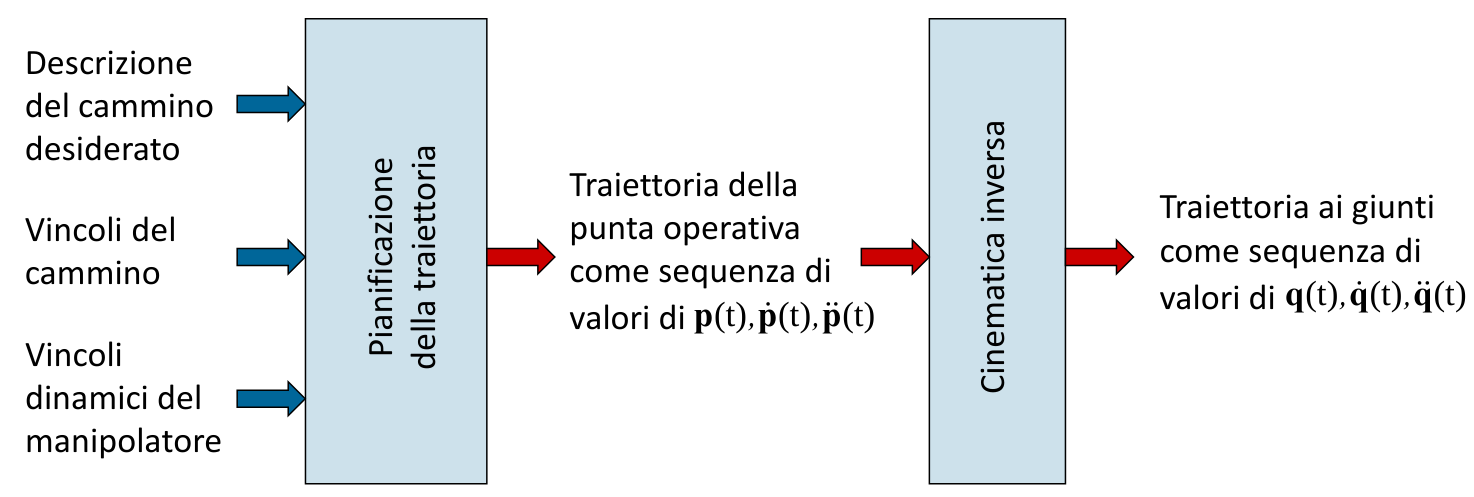
\includegraphics[width=0.9\linewidth]{images/trajectories_2}
	\caption{Flowpath}
	\label{fig:trajectories2}
\end{figure}

Path vs Trajectory:
\begin{itemize}
	\item Il \textbf{cammino (path)} è il luogo dei punti nello spazio dei giunti o nello spazio operazionale, che il manipolatore deve seguire durante l’esecuzione del movimento assegnato
	\item La \textbf{traiettoria (trajectory)} è un cammino sul quale è stata specificata una \textbf{legge temporale}, per esempio in termini di velocità ed accelerazioni in ogni suo punto
\end{itemize}

\begin{figure}[H]
	\centering
	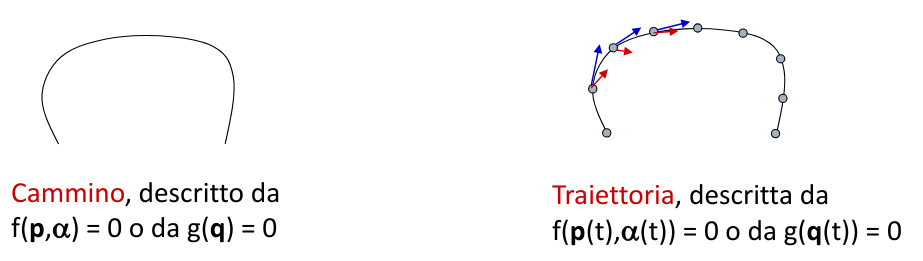
\includegraphics[width=0.7\linewidth]{images/trajectories_1}
	\caption{Path vs Trajectory}
	\label{fig:trajectories1}
\end{figure}

Il cammino desiderato viene specificato dall’utente per mezzo di un numero ridotto di parametri, quali punti estremi del cammino, eventuali punti intermedi, primitive geometriche di interpolazione. I requisiti sulla legge temporale sono principalmente legati a velocità ed accelerazioni massime.

\vspace*{10pt}
\textbf{Traiettorie nello spazio dei giunti o nello spazio operazionale?}
\begin{itemize}
	\item La pianificazione nello \textbf{spazio operazionale} è indicata ogni volta in cui sia necessario far seguire alla punta operativa un particolare percorso e/o sia necessario \textbf{evitare ostacoli} o zone “proibite” dello spazio di lavoro
	\item La pianificazione nello \textbf{spazio dei giunti} non consente di assegnare un particolare percorso alla punta, ma è utile per \textbf{evitare singolarità cinematiche} e/o per \textbf{sfruttare la ridondanza} del manipolatore, se presente
\end{itemize}






\section{Traiettorie nello spazio dei giunti}

In generale, devono comportare un basso sforzo computazionale e almeno posizioni e velocità devono essere funzioni continue del tempo (può essere interessante anche la continuità nell'accelerazione). Effetti indesiderati, come traiettorie non regolari per interpolare un dato insieme di punti, devono essere evitate.


\subsection{Point-to-Point (PTP) motion}
La traiettoria più semplice è quella corrispondente ad un\textbf{ movimento lineare da un punto ad un altro} (PTP - Point-To-Point) nello spazio dei giunti \textbf{(attenzione: il movimento cartesiano risultante è in generale NON lineare!)}.

Il manipolatore deve muoversi dalla configurazione iniziale $\bm{q}(t_0) = \bm{q}_0$ alla configurazione finale desiderata $\bm{q}(t_f) = \bm{q}_f$:
$$
\bm{q}(t_0) = \bm{q}_0 \quad \longrightarrow \quad \bm{q}(t_f) = \bm{q}_f
$$
rispettando i vincoli di velocità ed accelerazioni massime determinati dalle caratteristiche tecnologiche degli attuatori. \\
Eventuali vincoli sul \textit{jerk} (derivata dell’accelerazione rispetto al tempo) possono essere presenti per evitare sollecitazioni meccaniche eccessive. Si parla di movimento coordinato quando gli istanti di inizio e fine del moto coincidono per tutti i giunti.

Ovviamente esistono infinite soluzioni al problema sopra mostrato, possiamo però provare ad identificare quella ad energia minima. Immagina un manipolatore con giunti rotoidali, di conseguenza i movimenti saranno eseguiti attraverso delle coppie $\bm{\tau}$ fornite dai motori: possiamo provare a \textbf{minimizzare l'energia di tali motori}: imponendo $\dot{\bm{q}} = \bm{\omega}$ abbiamo ($F = ma \rightsquigarrow \tau = I\alpha$):
$$
\bm{\tau} = \bm{I}\dot{\bm{\omega}}
$$
dove $\bm{I}$ è il tensore d'inerzia del manipolatore. Quindi, volendo minimizzare l'energia:
\begin{align*}
	\text{minimize} \quad & \int_0^{t_f} \bm{\tau}^2(t)dt \\
	\text{subject to} \quad & \int_0^{t_f} \bm{\omega}(t)dt = \bm{q}_f - \bm{q}_i
\end{align*}
dove ricordiamo che $\int \bm{f}^2 = \text{energia}$.

Le \textbf{soluzioni} al problema sopra definito sono nella di un polinomio di 2° grado:
$$
\dot{\bm{q}}(t) = \bm{\omega}(t) = \alpha t^2 + \beta t + \gamma
$$
Dalla forma di $\dot{q}$ possiamo ricavare le forme di $q$ e $\ddot{q}$, che saranno rispettivamente polinomi di 3° grado e di 1° grado\footnote{se $\dot{\bm{q}}$ è un polinomio di 2° ordine, derivando per andare a $\ddot{\bm{q}}$ otteniamo un poly di 1° ordine, mentre integrando per andare a $\bm{q}$ otteniamo un poly di 3° ordine}. Per comodità di notazione indichiamo analiticamente i coefficienti di $q$, e poi deriviamo per ottenere gli altri:
\begin{equation}\label{eq:cubic_sol_traj}
\begin{aligned}
	\bm{q}(t) &= a_3t^3 + a_2t^2 + a_1t + a_0 \\
	\bm{\dot{q}}(t) &= 3a_3t^2 + 2a_2t + a_1 \\
	\bm{\ddot{q}}(t) &= 6a_3t + 2a_2
\end{aligned}
\end{equation}
(\textit{per capire meglio, rispetto alla notazione di prima abbiamo} $\alpha=3a_3, \ \beta = 2a_2, \ \gamma = a_1$).

Di seguito vediamo un esempio di traiettoria:
\begin{figure}[H]
	\begin{subfigure}{0.3\linewidth}
		\centering
		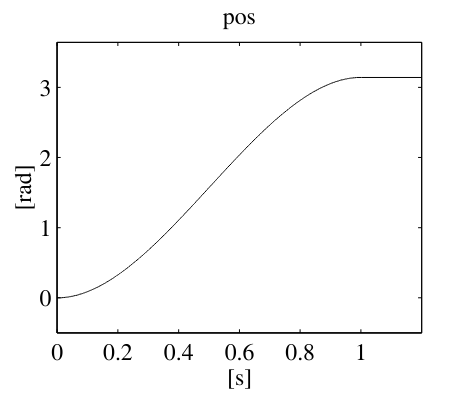
\includegraphics[width=\linewidth]{images/trajectories_4}
		\caption{Posizione}
		\label{fig:trajectories4}
	\end{subfigure}
	\hfill
	\begin{subfigure}{0.3\linewidth}
		\centering
		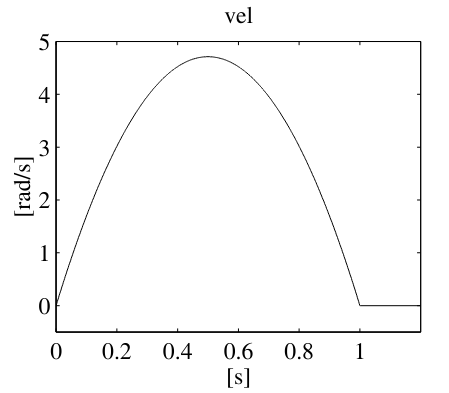
\includegraphics[width=\linewidth]{images/trajectories_5}
		\caption{Velocità}
		\label{fig:trajectories5}
	\end{subfigure}
	\hfill
	\begin{subfigure}{0.3\linewidth}
		\centering
		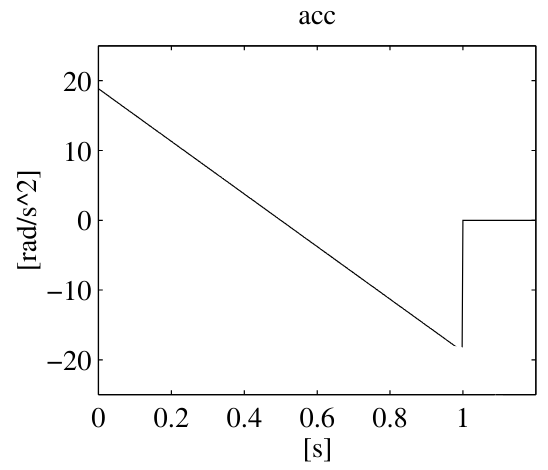
\includegraphics[width=\linewidth]{images/trajectories_6}
		\caption{Accelerazione}
		\label{fig:trajectories6}
	\end{subfigure}	
	\caption{Esempio}
\end{figure}
\vspace*{-9pt}
notare come l'accelerazione non è continua per $t = 1$: fortunatamente a quell'istante di tempo $v = 0$ e quindi non ci sono problemi.



\vspace*{10pt}
\subsubsection{Soluzione generale}
Quindi, come impostiamo i nostri requisiti? Visto che abbiamo 4 coefficienti ($a_4, \dots, a_0$) possiamo imporre 4 grandezze: nel caso seguente imporremo posizione iniziale e finale, e velocità iniziale e finale (che solitamente sono imposte a $0$):
$$
\begin{cases*}
	\bm{q}(t_i) = a_3t_i^3 + a_2t_i^2 + a_1t_i + a_0 \\
	\bm{q}(t_f) = a_3t_f^3 + a_2t_f^2 + a_1t_f + a_0 \\
	\bm{\dot{q}}(t_i) = 3a_3t_i^2 + 2a_2t_i + a_1 \\
	\bm{\dot{q}}(t_i) = 3a_3t_f^2 + 2a_2t_f + a_1 \\
	\bm{q}(t_i) = \bm{q}_i \\
	\bm{q}(t_f) = \bm{q}_f \\
	\bm{\dot{q}}(t_f) = \bm{\dot{q}}_i \\
	\bm{\dot{q}}(t_f) = \bm{\dot{q}}_f
\end{cases*}
$$

Visto che solitamente $t_i = 0$, otteniamo:
$$
\boxed{
\begin{cases*}
	\bm{q}_i = a_0 \\
	\bm{q}_f = a_3t_f^3 + a_2t_f^2 + a_1t_f + a_0 \\
	\bm{\dot{q}}_i = a_1 \\
	\bm{\dot{q}}_f = 3a_3t_f^2 + 2a_2t_f + a_1
\end{cases*}
}
$$
dove, imponendo i nostri requisiti di $q_i,q_f,	\dot{q}_i,\dot{q}_f$ otteniamo i coefficienti per i 3 polinomi.



\vspace*{10pt}
\subsubsection{Alternativa per assegnare l'accelerazione}
Abbiamo visto che una soluzione della forma (\ref{eq:cubic_sol_traj}) ci garantisce la minimizzazione dell'energia dei motori, putroppo però abbiamo a disposizione solo 4 coefficienti, quindi non c'è modo (ad esempio) di impostare l'accelerazione. Se vogliamo assegnare anche $\ddot{\bm{q}}_f, \ \ddot{\bm{q}}_i$ ci servono 4 coefficienti, ovvero:
$$
\bm{q}(t) = a_5t^5 + a_4t^4 + a_3t^3 + a_2t^2 + a_1t + a_0
$$
N.B. una soluzione di questo tipo \underline{non} minimizza l'energia.



\vspace*{10pt}
\subsection{Profilo di velocità trapezoidale (2-1-2)}

Anche chiamata LSPB (\textit{linear segment paraboloid blend}), questa è una traiettoria molto frequente nelle applicazioni industriali, vista la sua semplicità di implementazione. Inoltre permette di verificare che le velocità e le accelerazioni siano compatibili con le caratteristiche fisiche del manipolatore (visto che se ne possono impostare minimi/massimi facilmente).

L'idea alla base è di imporre un profilo \textbf{trapezoidale} alla velocità, ovvero accellerazione costante all'inizio e alla fine e nulla nel mezzo (i.e velocità lineare all'inzio/fine e costante nel mezzo).

\begin{figure}[H]
	\centering
	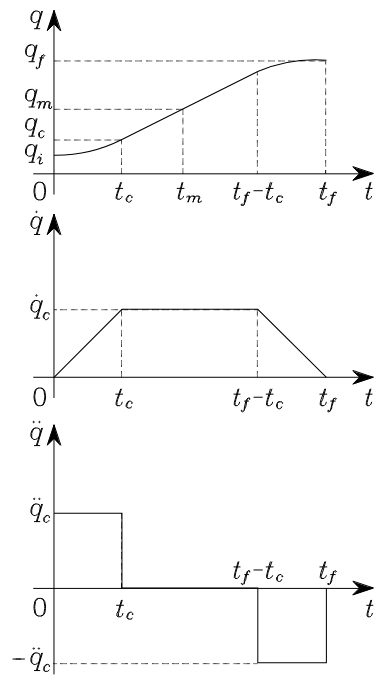
\includegraphics[width=0.3\linewidth]{images/trajectories_7}
	\caption{Esempio}
	\label{fig:trajectories7}
\end{figure}

Visto che (in generale) supponiamo velocità iniziale/finale nulle e durata dei periodi di accelerazione uguale, otteniamo traiettorie simmetriche rispetto ad un punto di mezzo, che è dato da:
$$
t_m = \frac{t_f}{2}
\qquad , \qquad
\bm{q}_m = \frac{\bm{q}_f + \bm{q}_i}{2}
$$


\vspace*{10pt}
\subsubsection{Calcolo dei valori di velocità e accelerazione}
Solitamente, per questo tipo di profilo viene dato il tempo finale $t_f$ (ovvero, visto che in generale $t_i = 0$, viene dato il tempo desiderato per eseguire la traiettoria). Da questo vincolo però dobbiamo trovarci i corretti valori di velocità che ci assicurano un passaggio da $q_i$ a $q_f$ nel tempo dato $t_f$.

In primis possiamo vedere che la veloctià di crociera (i.e. quella costante) $\bm{\dot{q}}_c$ è data da:
$$
\bm{\dot{q}}_c 
= 
\frac{\bm{q}_m - \bm{q}_c}{t_m - t_c}
=
\frac{\text{rise}}{\text{run}}
$$
dove $\bm{q}_c$ e $t_c$ sono rispettivamente l'angolo e il tempo in cui inizia la fase di crociera. La formula può essere facilmente capita anche guardando l'immagine di seguito.

\begin{figure}[H]
	\centering
	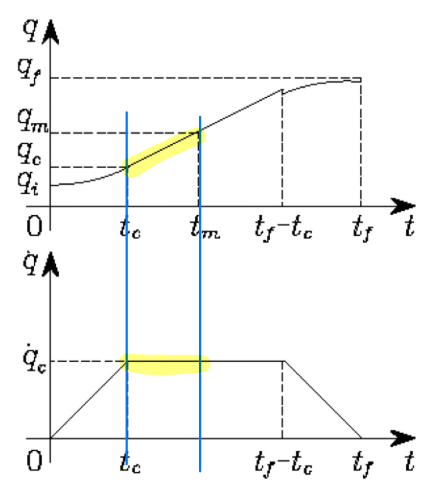
\includegraphics[width=0.35\linewidth]{images/trajectories_8}
	\label{fig:trajectories8}
\end{figure}

Ora, per quanto riguarda l'accelerazione, abbiamo il seguente vincolo (richiamando $v = at$):
$$
\bm{\ddot{q}}t_c
=
\bm{\dot{q}}
=
\frac{\bm{q}_m - \bm{q}_c}{t_m - t_c}
$$
\begin{figure}[H]
	\centering
	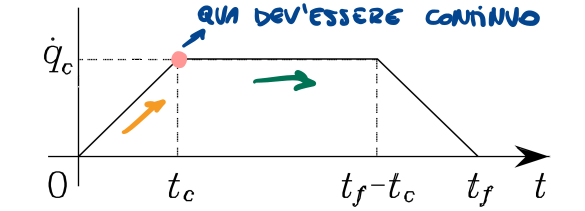
\includegraphics[width=0.4\linewidth]{images/trajectories_9}
	\label{fig:trajectories9}
\end{figure}
Inoltre, ricordando fisica 1, possiamo esprimere il valore di $q_c$ tramite la legge di moto rettilineo uniformemente accelerato:
$$
x = x_0 + \frac{1}{2}at^2
\implies
\bm{q}_c = \bm{q}_i + \frac{1}{2}\bm{\ddot{q}}_ct_c^2
$$
Concludendo, combinando le ultime due equazioni abbiamo:
$$
\bm{\ddot{q}}_ct_c^2
+
\bm{\ddot{q}}_c t_f t_c
+
\bm{q}_f - \bm{q}_i = 0
$$
Questa equazione può ora essere risolta per ottenere $t_c$. In particolare di solito per risolverla si assegna il seguente constraint:
$$
\text{sgn}(\ddot{\bm{q}})
=
\text{sgn}(\bm{q}_f - \bm{q}_i)
$$
Quindi, dati $t_f, \ \bm{q}_i, \ \bm{q}_f$ troviamo:
\begin{equation}\label{eq:tc_212}
\boxed{
t_c
=
\frac{t_f}{2} - \frac{1}{2}
\sqrt{
\frac{t_f^2 \ddot{\bm{q}} - 4(\bm{q}_f - \bm{q}_i)}{\bm{\ddot{q}}_c}
}
}
\end{equation}
vista la forma della soluzione, abbiamo ulteriori vincoli (dati dal segno del fattore sotto radice):
\begin{equation}\label{eq:qddot_constraint_212}
|\ddot{\bm{q}}| \ge \frac{4|\bm{q}_f - \bm{q}_i|}{t_f^2}
\end{equation}
Conoscere il valore di $t_c$ ci permette di disegnare il controllo per la traiettoria terminando la fase di accelerazione ed iniziando quella di decelerazione ai tempi ora noti.

\vspace*{10pt}
\subsubsection{Bang-Bang controller}
Nel caso particolare in cui
$$
t_c = \frac{t_f}{2}
$$
(solitamente abbiamo $\leq$ invece di $=$), otteniamo un controllore "bang-bang", ovvero con \textbf{profilo triangolare di velocità}. Il nome deriva dal fatto che i motori sono attuati o al massimo o sono spenti
\begin{figure}[H]
	\centering
	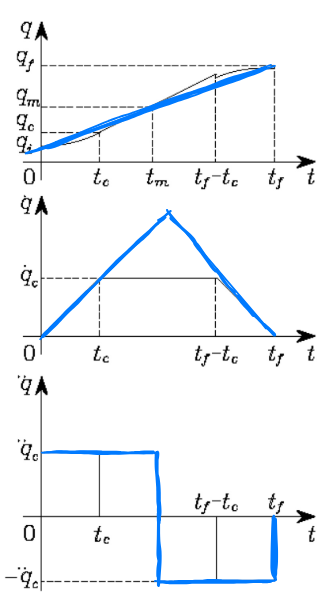
\includegraphics[width=0.3\linewidth]{images/trajectories_10}
	\caption{Esempio bang-bang}
	\label{fig:trajectories10}
\end{figure}



\vspace*{10pt}
\subsubsection{Soluzione profilo trapezoidale}
Per concludere, vediamo come si ottengono valori di $\bm{q}(t)$ noti $t_f$, $q_i$ e $q_f$. Calcolando $t_c$ con (\ref{eq:tc_212}) prima e scegliendo un $\ddot{\bm{q}}$ che rispetta il vincolo (\ref{eq:qddot_constraint_212}) abbiamo:

$$
\boxed{
\bm{q}(t)
=
\begin{cases}
\bm{q}_i + \frac{1}{2} \ddot{\bm{q}}_c t^2 & \quad 0 \leq t \leq t_c \\
\bm{q}_i + \ddot{\bm{q}}_c t_c (t - t_c/2) & \quad t_c < t \leq t_f - t_c \\
\bm{q}_i - \frac{1}{2} \ddot{\bm{q}}_c (t_f - t)^2 & \quad t_f - t_c < t \leq t_f
\end{cases}
}
$$



\begin{example}
Dati
$$
(q_i, q_f, t_i, t_f, \ddot{q}_c)
=
(0,\pi,0,1,6\pi)
$$
visto che
$$
\frac{4|q_f - q_i|}{t_f^2} = 4\pi
$$
la scelta di $\ddot{q} = 6\pi$ è corretta. Ora usando le formule viste:
$$
t_c = \frac{1}{2} - \frac{1}{2}\sqrt{\frac{\pi}{3}} = 0.12
$$
e quindi:
$$
q(t)
=
\begin{cases}
	3\pi t^2 & \quad 0 \leq t \leq 0.12 \\
	0.72\pi (t - 0.06) & \quad 0.12 < t \leq 0.88 \\
	\pi - 3\pi (1 - t)^2 & \quad 0.88 < t \leq 1
\end{cases}
$$



\vspace*{10pt}
\begin{figure}[H]
	\begin{subfigure}{0.3\linewidth}
		\centering
		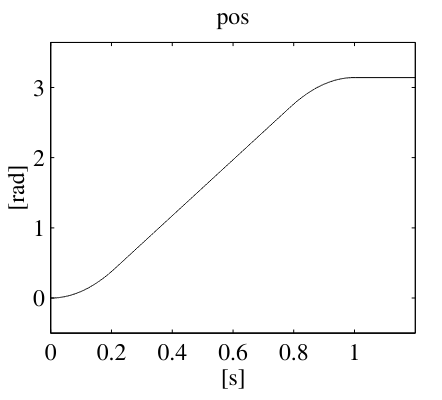
\includegraphics[width=\linewidth]{images/trajectories_12}
		\caption{Posizione}
		\label{fig:trajectories12}
	\end{subfigure}
	\hfill
	\begin{subfigure}{0.3\linewidth}
		\centering
		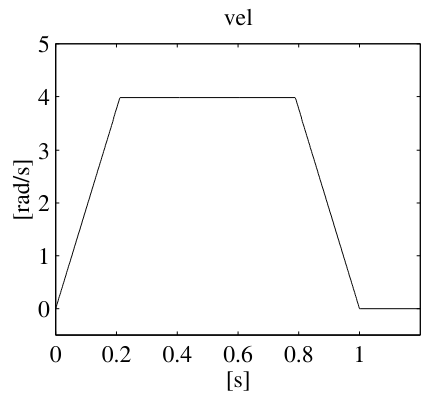
\includegraphics[width=\linewidth]{images/trajectories_13}
		\caption{Velocità}
		\label{fig:trajectories13}
	\end{subfigure}
	\hfill
	\begin{subfigure}{0.3\linewidth}
		\centering
		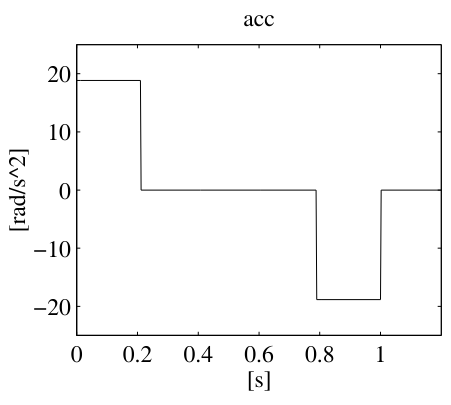
\includegraphics[width=\linewidth]{images/trajectories_14}
		\caption{Accelerazione}
		\label{fig:trajectories14}
	\end{subfigure}	
	\caption{Esempio}
\end{figure}
\end{example}




\vspace*{10pt}
\subsubsection{Assegnazione della velocità di crociera}
Sfruttando le formule note invece di assegnare l'accelerazione, possiamo ottenere il valore di $\bm{\ddot{q}}_c$ da $\bm{\dot{q}}_c$, di fatto assegnando la velocità invece dell'accelerazione:
\begin{figure}[H]
	\centering
	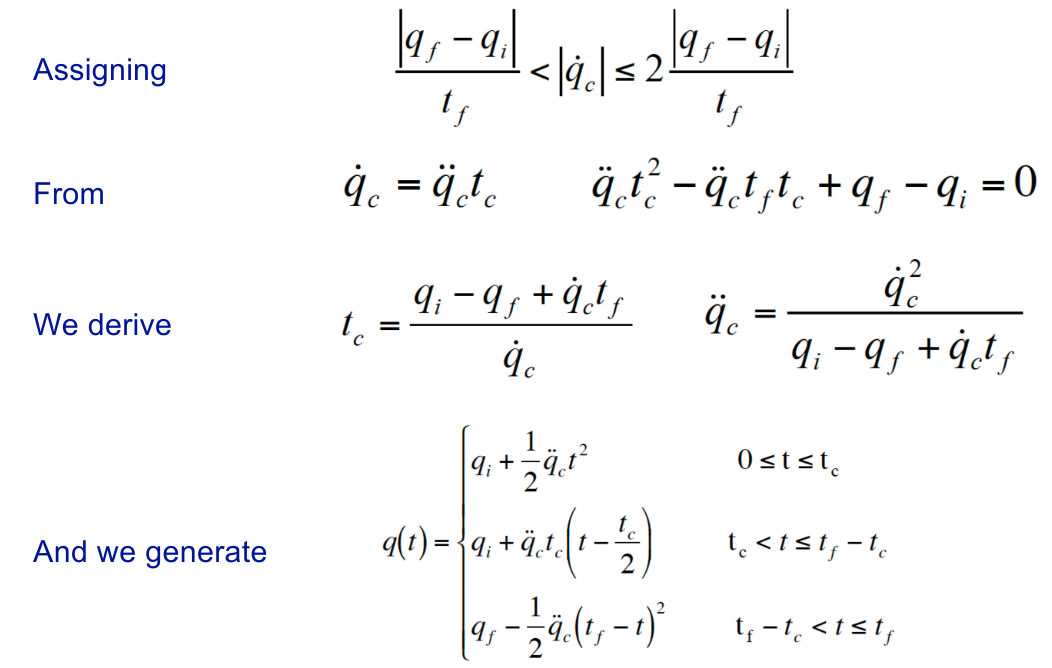
\includegraphics[width=0.9\linewidth]{images/trajectories_15}
	\label{fig:trajectories15}
\end{figure}



\vspace*{10pt}
\subsubsection{Comparazione con PTP}
Visto che questa soluzione non minimizza l'energia, abbiamo ovviamente una soluzione peggiore da quel punto di vista, anche se non di troppo (circa 12.5\% peggio). Come già accennato questo profilo è molto usato perchè semplice da implementare e leggero dal punto di vista computazionale.





\vspace*{15pt}
\subsection{Movimento attraverso una sequenza di punti}
In caso di compiti complessi, la traiettoria è specificata da una sequenza di punti (configurazioni $\bm{q}_k$) che il manipolatore deve raggiungere in determinati istanti di tempo \hl{bla bla bla TODO}
